  \begin{frame}{Plasma und kosmische Magnetfelder}
    \begin{columns}
   \begin{column}{0.5\textwidth}
    \begin{itemize}
      \setlength\itemsep{2em}
      \item  Plasma: vollständiges oder teilweise ionisiertes Gas\\[1.5em]
            $\longrightarrow$ Enthält Ladung
      \item  Plasma kann Magnetfelder mit sich führen
      \item  Beobachtbar mithilfe polarisierter Radiostrahlung
    \end{itemize}
  \vspace{2em}
  \end{column}
  \begin{column}{0.5\textwidth}
  \begin{figure}
    \centering
    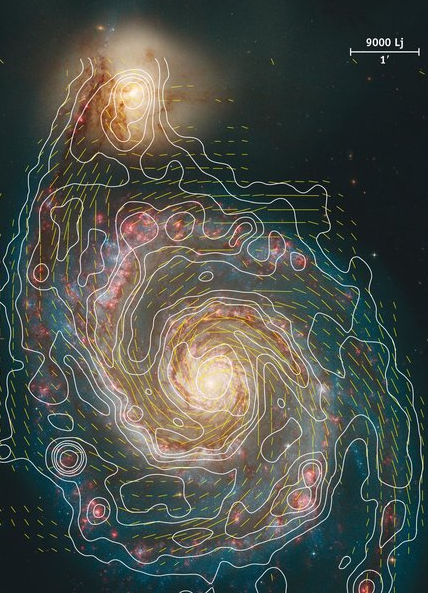
\includegraphics[width=0.6\textwidth]{images/magnetfelder.png}
  \end{figure}
  \end{column}
    \end{columns}
  \end{frame}

  \begin{frame}{Was zeichnet einen unipolaren Induktor und was eine magnetische Rekonnektion aus?}
    \begin{columns}
   \begin{column}{0.5\textwidth}
    \begin{itemize}
      \setlength\itemsep{2em}
      \item  Unipolarinduktion: Trennung von elektrischer Ladung mithilfe des magnetischen Teiles der Lorentzkraft\\[1.5em]
            $\longrightarrow$ Elektrische Spannung entsteht
      \item  Magnetische Rekonnektion: Struktur des Magnetfelds ändert sich abrupt und es werden große Energiemengen freigesetzt
    \end{itemize}
  \vspace{2em}
  \end{column}
  \begin{column}{0.5\textwidth}
  \begin{figure}
    \centering
    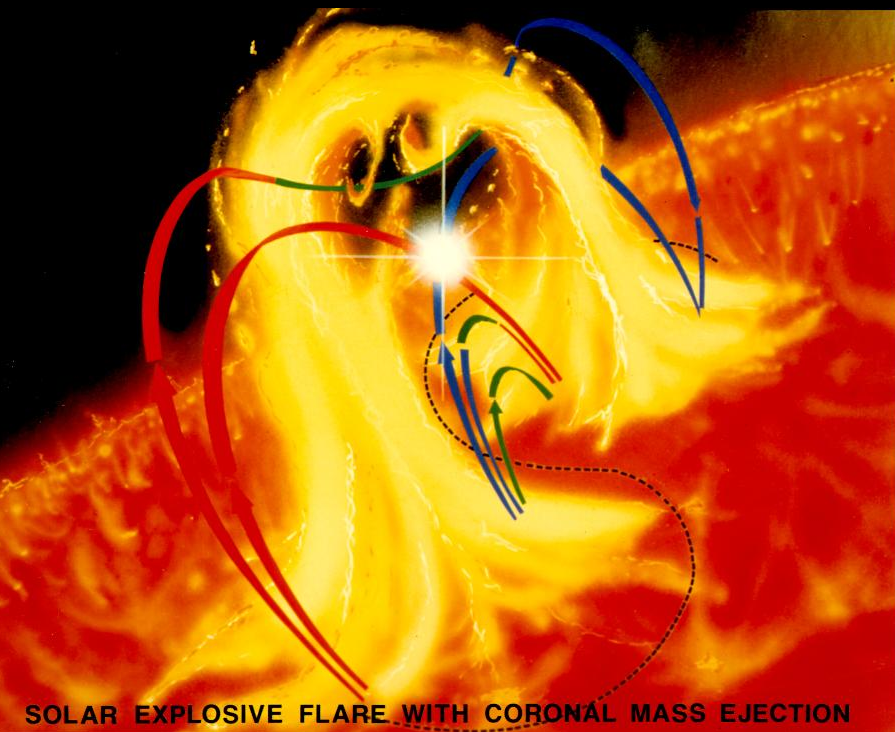
\includegraphics[width=0.6\textwidth]{images/rekonnektion.png}
  \end{figure}
  \end{column}
    \end{columns}
  \end{frame}


  \begin{frame}{Wie kann erkannt werden, wodurch Cherenkovstrahlung entsteht und welche ist von Interesse?\\
  Wie genau funktioniert die Detektion von Cherenkovstahlung mittels Teleskopen?\\
  Woher weiß man, ob die Gammastrahlung kosmischen Ursprungs ist?}
    \begin{columns}
   \begin{column}{0.5\textwidth}
    \begin{itemize}
      \setlength\itemsep{2em}
      \item  Hochenergetische Gammastrahlung trifft auf Atmosphäre $\rightarrow$ Teilchenschauer entsteht
      \item  Elektronen bewegen sich mit Geschwindigkeiten größer als Lichtgeschwindigkeit im Medium $\rightarrow$ Cherenkovstrahlung entsteht
      \item  Cherenkovteleskope beobachten in Quellrichtung, initialer Schauer wird in Kamera abgebildet $\rightarrow$ Schauerellipsen\\[1.5em]
            $\longrightarrow$ Rückschlüsse auf Richtung und Energie des Ursprungsteilchen

    \end{itemize}
  \vspace{2em}
  \end{column}
  \begin{column}{0.5\textwidth}
  \begin{figure}
    \centering
    \includegraphics[width=0.5\textwidth]{images/magic.JPG}\\
    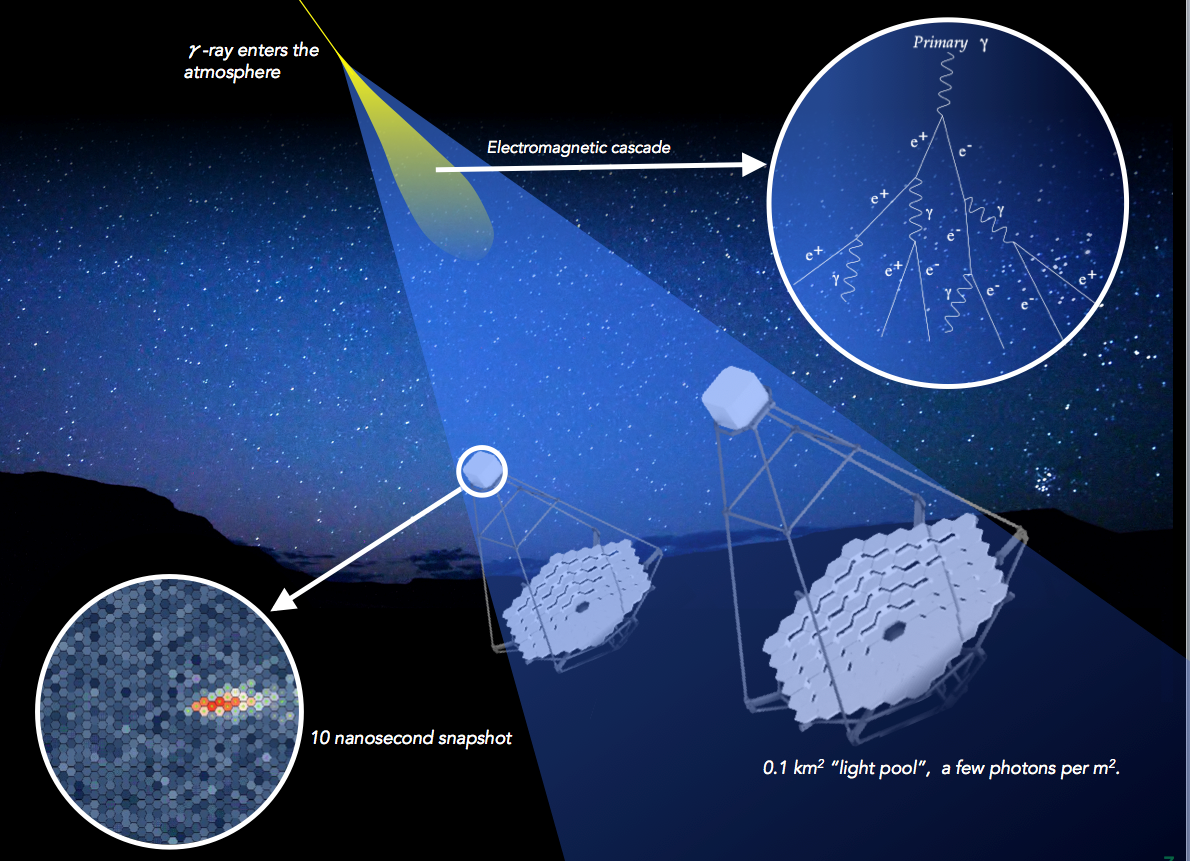
\includegraphics[width=0.5\textwidth]{images/cta_schauer.png}
  \end{figure}
  \end{column}
    \end{columns}
  \end{frame}


  \begin{frame}{Wie und wo entstehen Gravitationswellen?}
    \begin{columns}
   \begin{column}{0.5\textwidth}
    \begin{itemize}
      \setlength\itemsep{2em}
      \item Verschmelzung/Umkreisung zweier massereicher Objekte
      \item Gravitationspotential ändert sich bis zur finalen Verschmelzung
      \item Bei Verschmelzung: Gravitationspotential kann sich nicht abrupt ändern $\rightarrow$ Änderung breitet sich mit Lichtgeschwindigkeit aus
      \item Entstehung von Wellenmuster im Raum
     \end{itemize}
  \vspace{2em}
  \end{column}
  \begin{column}{0.5\textwidth}
  \begin{figure}
    \centering
    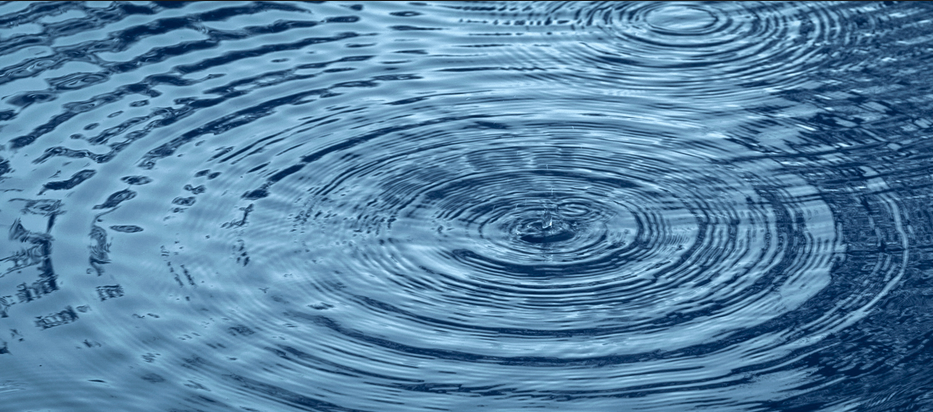
\includegraphics[width=0.6\textwidth]{images/welle.png}\\
    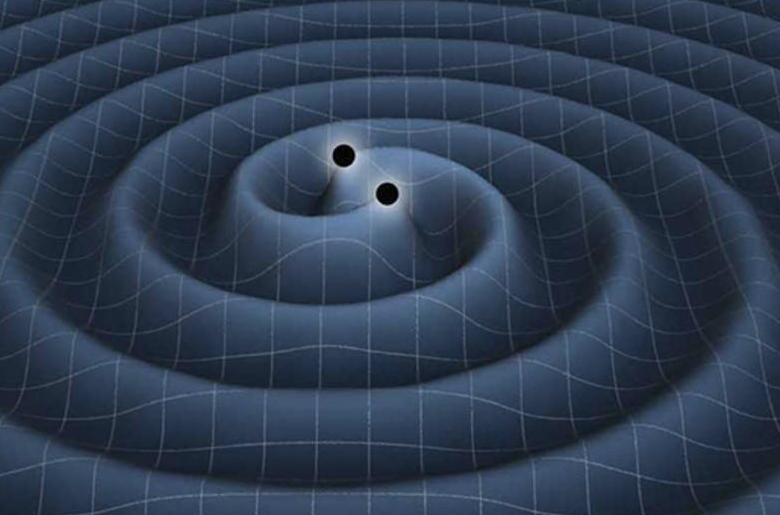
\includegraphics[width=0.6\textwidth]{images/welle2.png}
  \end{figure}
  \end{column}
    \end{columns}
  \end{frame}

  \begin{frame}{Wie funktioniert die Sternstromparallaxe?}
    \begin{columns}
   \begin{column}{0.5\textwidth}
    \begin{itemize}
      \setlength\itemsep{2em}
      \item Wird auf Hyaden im Sternenbild Stier angewendet
      \item Parallele Raumgeschwindigkeit vom gleichen Betrag
      \item Bewegen sich auf Konvergenzunkt zu (Beteigeuze im Sternbild Orion)
      \item Basis der galaktischen und intergalaktischen Entfernungsskala
     \end{itemize}
  \vspace{2em}
  \end{column}
  \begin{column}{0.5\textwidth}
  \begin{figure}
    \centering
    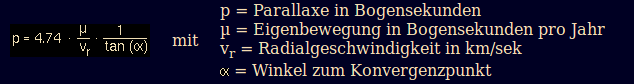
\includegraphics[width=\textwidth]{images/sternstromparallaxe.png}
  \end{figure}
  \end{column}
    \end{columns}
  \end{frame}


  \begin{frame}{Was genau ist der Fermimechanismus 1. und 2. Ordnung?}

    \begin{itemize}
      \setlength\itemsep{2em}
      \item Fermie 1. Ordnung:\\[1em]
            Beschleunigung eines geladenen Teilchens an einer Schockfront
      \item Fermie 2. Ordnung:\\[1em]
            Streuung eines relativistischen geladenen Teilchens an einer Plasmawolke
     \end{itemize}

  \end{frame}

  \begin{frame}{Was ist der Lyman-α-Wald?\\
    Wie kann interstellare Materie genau nachgewiesen werden bzw. wie funktioniert der Nachweis?}
    \begin{columns}
   \begin{column}{0.5\textwidth}
    \begin{itemize}
      \setlength\itemsep{2em}
      \item Ly-$\alpha$-Übergang im neutralen Wasserstoff
      \item Absorption von Licht in intergalaktischen Gaswolken
      \item Durchgang des Lichts bei unterschiedlichen Rotverschiebungen
      \item Scharfe Absorptionslinien im Spektrum von Quasaren
      \item Rückschluss auf Dichte der Wolken im Universum
     \end{itemize}
  \vspace{2em}
  \end{column}
  \begin{column}{0.5\textwidth}
  \begin{figure}
    \centering
    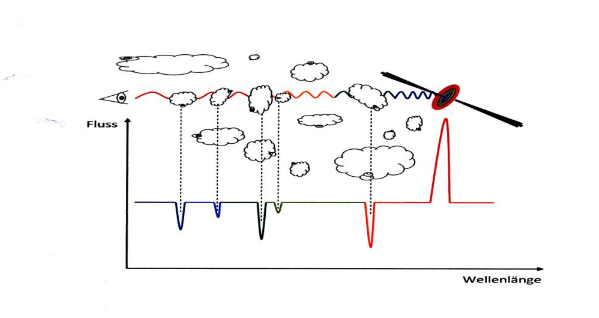
\includegraphics[width=\textwidth]{images/lawald.png}
  \end{figure}
  \end{column}
    \end{columns}
  \end{frame}

  \begin{frame}{Was/Wofür ist das Fireball-Modell?}
    \begin{columns}
   \begin{column}{0.5\textwidth}
    \begin{itemize}
      \setlength\itemsep{2em}
      \item Erklärung für hohe Energie und kurze Zeitskalen von GRBs
      \item Initialer Burst und ausgedehntes Nachleuchten
      \item Große Variabilität der Flüsse schließen auf kleine Emissionsregionen
     \end{itemize}
  \vspace{2em}
  \end{column}
  \begin{column}{0.5\textwidth}
  \begin{figure}
    \centering
    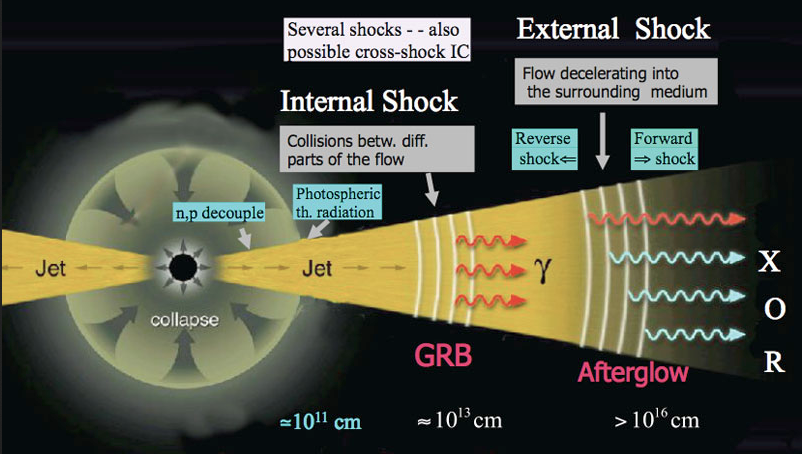
\includegraphics[width=\textwidth]{images/fireball.png}
  \end{figure}
  \end{column}
    \end{columns}
  \end{frame}

  \begin{frame}{Was genau zeichnet den Fluss kosmischer Strahlung aus?\\
  Bei der Untersuchung von CR ist ja ein Ziel die Lorentzverletzung zu
  zeigen, aber wie will man das tun? Wonach sucht man?}
    \begin{columns}
   \begin{column}{0.5\textwidth}
    \begin{itemize}
      \setlength\itemsep{2em}
      \item Besteht aus unterschiedlichen Teilechen
      \item Auf lange Sicht konstanter Fluss
      \item Lorentzverletzung:\\[1em]
      Photonen hätten eine energieabhängige Geschwindigkeit\\[1em]
      Photonen mit Energien von $\SI{e19}{\electronvolt}$ wären stark unterdruck\\[1em]
      Wurde vom Auger Experiment nicht nachgewiesen
     \end{itemize}
  \vspace{2em}
  \end{column}
  \begin{column}{0.5\textwidth}
  \begin{figure}
    \centering
    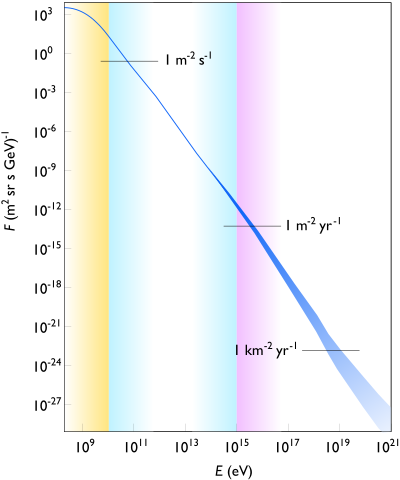
\includegraphics[width=0.7\textwidth]{images/cr.png}
  \end{figure}
  \end{column}
    \end{columns}
  \end{frame}

  \begin{frame}{Wie ist der Mikrowellenhintergrund zu erklären, wo entsteht die Strahlung
  und wie kann sie die Erde erreichen, wenn sich alles vom Zentrum des Urknalls
  wegbewegt?\\
    Wie lässt sich der Ursprung der kosmischen Hintergrundstrahlung verstehen?\\
    Wodurch genau kommt die 3K Hintergrundstrahlung zustande? Wie genau wurde die Struktur des kosmischen Mikrowellenhintergrunds bestimmt?
    Und warum/wofür wird das zugehörige Spektrum untersucht?}
    \begin{columns}
   \begin{column}{0.5\textwidth}
    \begin{itemize}
      \setlength\itemsep{1em}
      \item Überbleibsel des Urknalls
      \item Erst undurchsichtiges Plasma $\rightarrow$ ab $z=1100$ Universum durchsichtig, Elektronen entkoppeln
      \item Neuste Messungen mit dem Planck-Satelliten
      \item Genauigkeit: 4 Bogenminuten für die höchsten und 33 Bogenminuten für die niedrigsten Frequenzen
      \item Spektrum gibt Rückschluss auf Materieverteilung im Universum und kosmologische Konstanten
     \end{itemize}
  \vspace{2em}
  \end{column}
  \begin{column}{0.5\textwidth}
  \begin{figure}
    \centering
    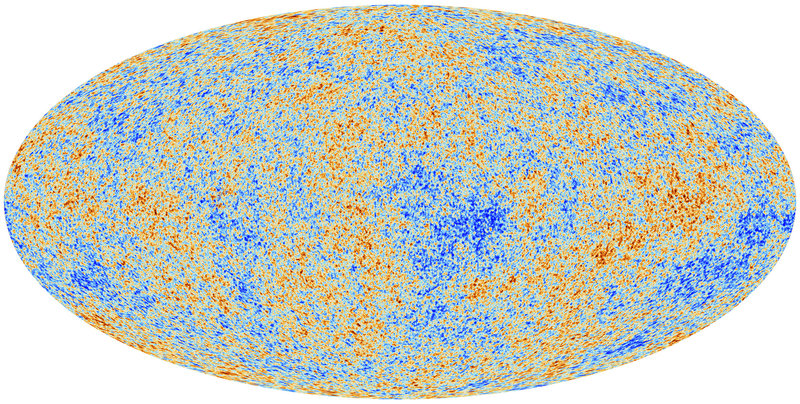
\includegraphics[width=\textwidth]{images/planck.jpg}
  \end{figure}
  \end{column}
    \end{columns}
  \end{frame}

  \begin{frame}{Wie spektroskopiert man Das Licht von astronomischen Quellen? Mit einem Prisma, oder wird das irgendwie gesamplet und digitalisiert?}
    \begin{columns}
   \begin{column}{0.5\textwidth}
    \begin{itemize}
      \setlength\itemsep{2em}
      \item Zur Auffächerung des Spektrums kann ein Prisma oder ein Gitter verwendet werden
      \item Anschließend wird das Spektrum mit einer CCD-Kamera digitalisiert
      \item In Radioastronie wird größerer Frequenzbereich betrachtet und Signal in verschiedene Frequenzbins eingeteilt
     \end{itemize}
  \vspace{2em}
  \end{column}
  \begin{column}{0.5\textwidth}
  \begin{figure}
    \centering
    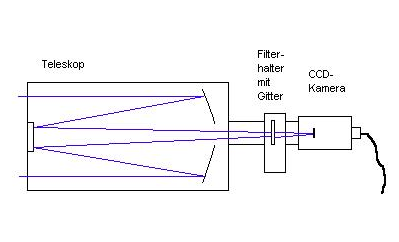
\includegraphics[width=0.6\textwidth]{images/spektroskopie.png}\\
    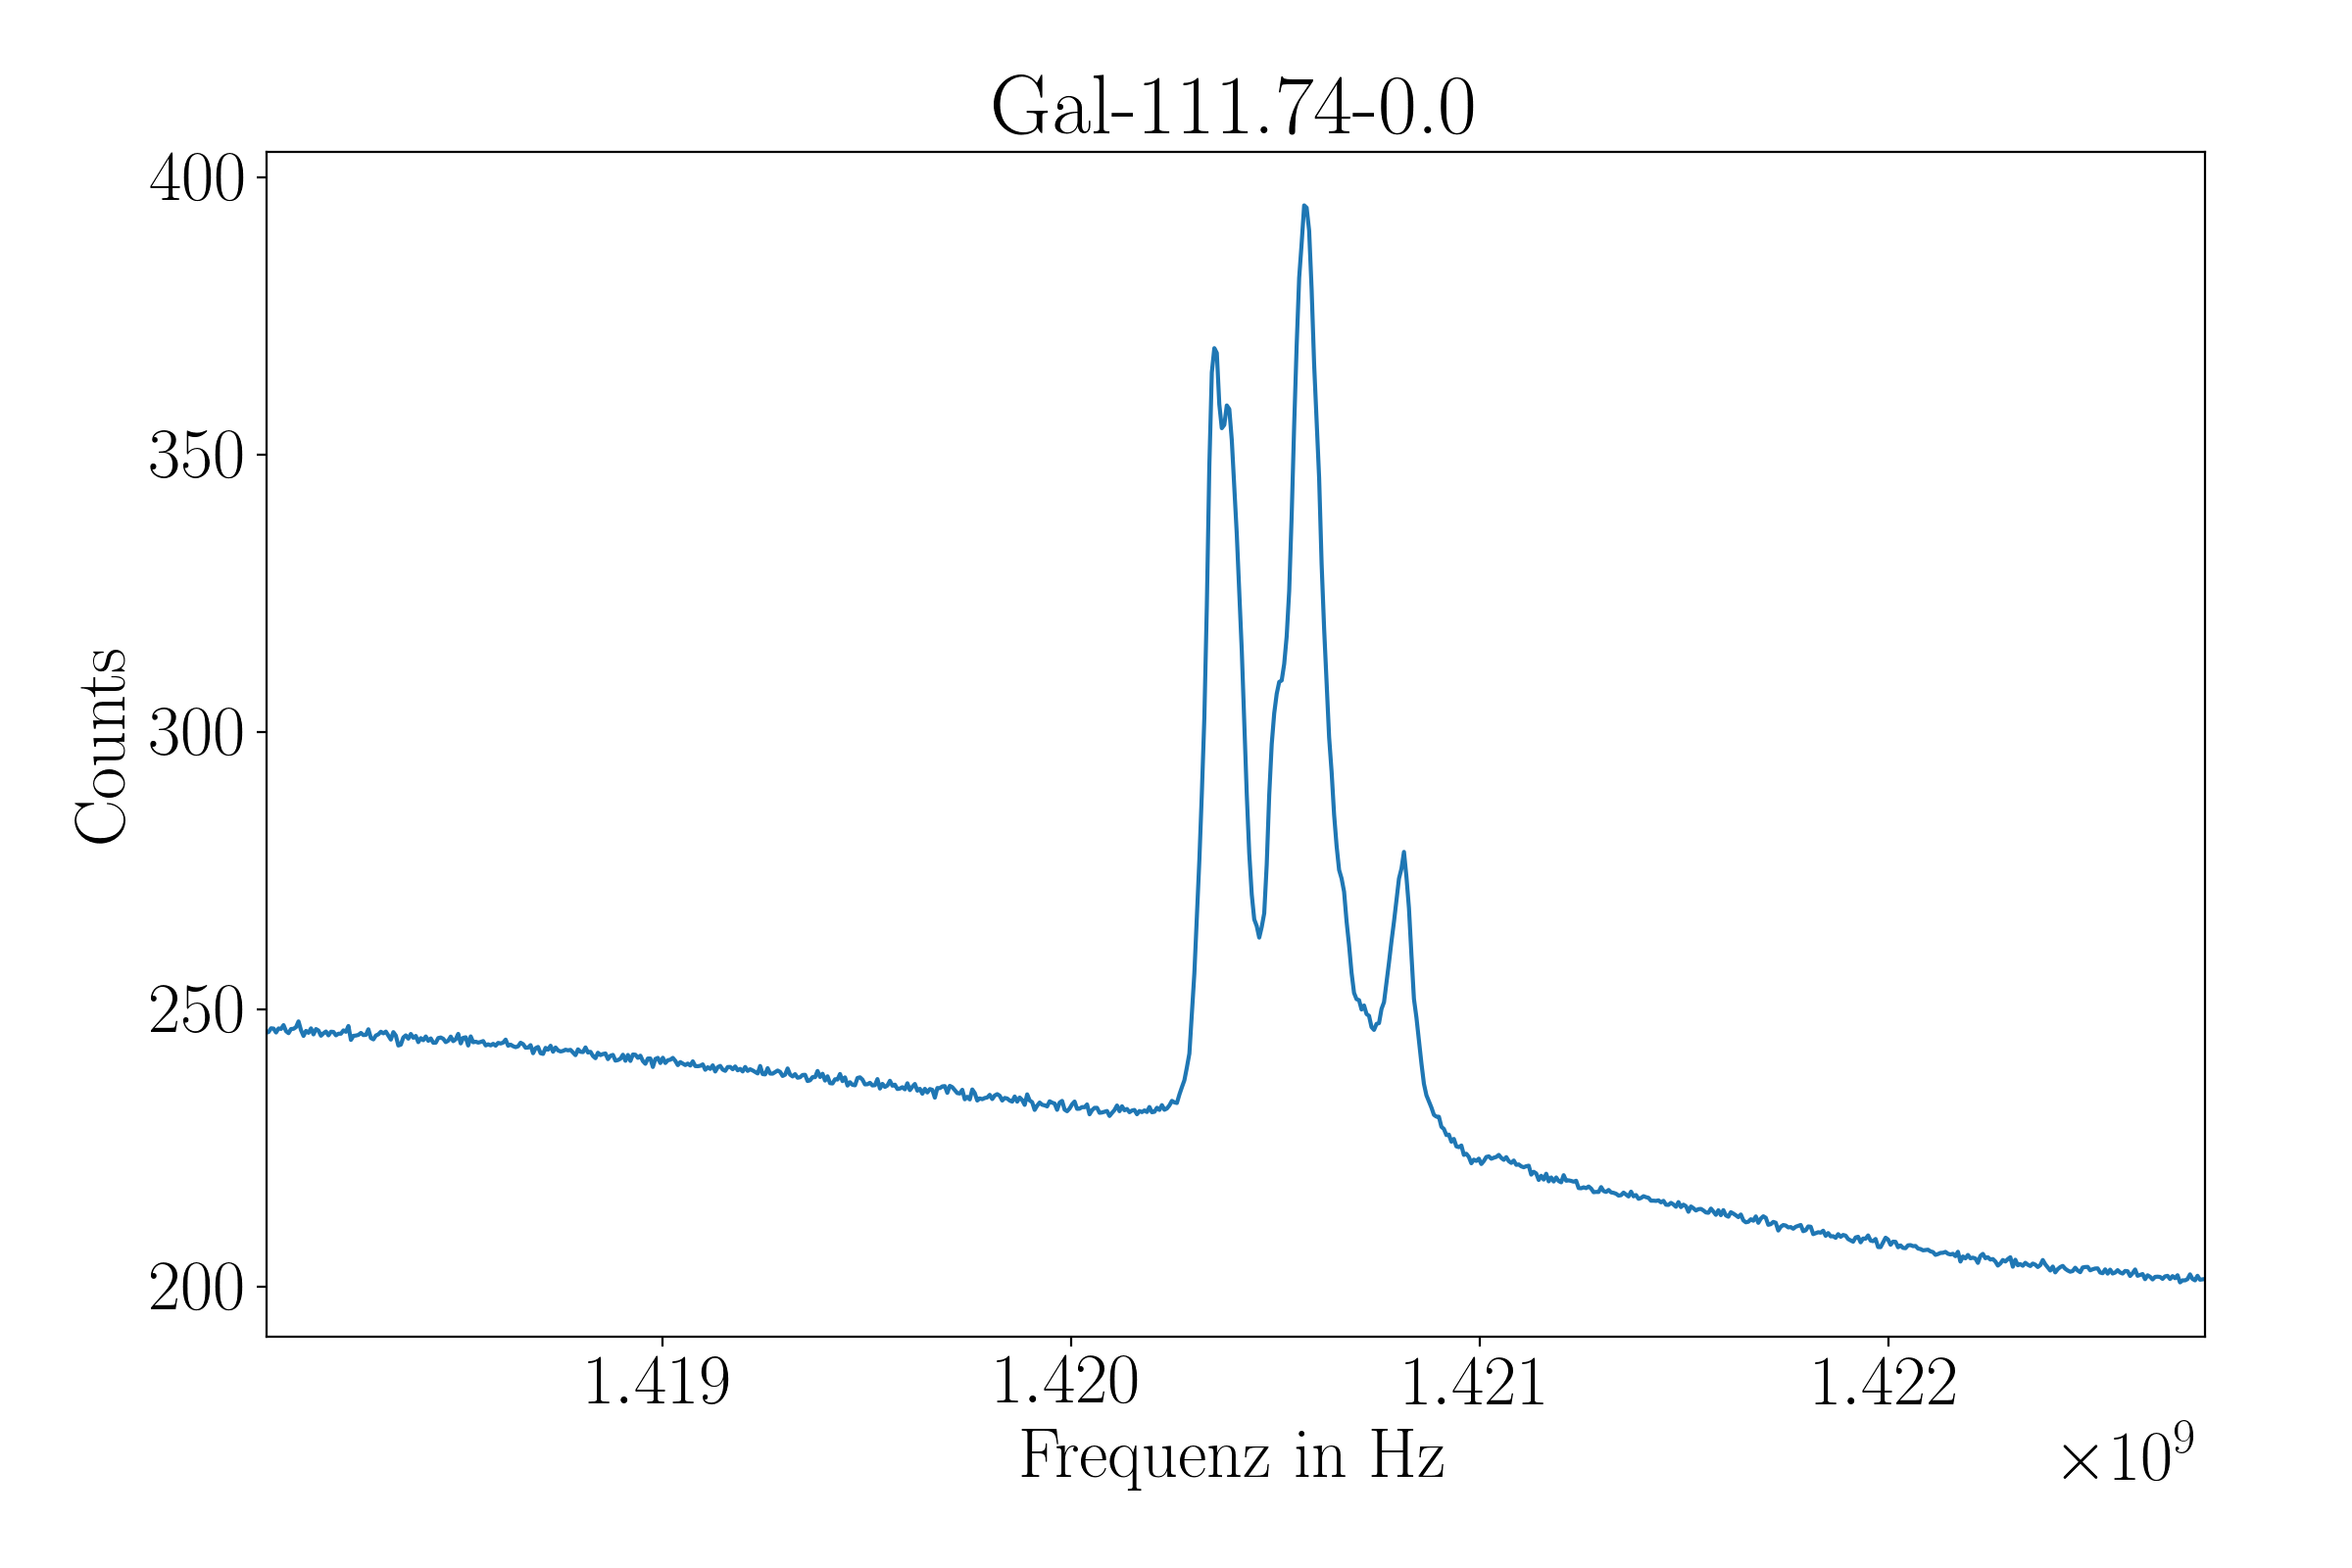
\includegraphics[width=0.8\textwidth]{images/gal_111_addiert.png}
  \end{figure}
  \end{column}
    \end{columns}
  \end{frame}

  \begin{frame}{Noch mehr Fragen...}

    \begin{itemize}
      \setlength\itemsep{2em}
      \item Wie bekommt man es hin, dass moderne Teleskope eine so gute Auflösung
            besitzen (zb. Hubble Teleskop :0,05")?\\[1em]
            $\sin(\delta) = 1.22\frac{\lambda}{D}$
      \item Woher kommen die unterschiedlich geschätzten Lebensdauern von Protonen?\\[1em]
            Protonen sind stabil, man kann die Lebensdauer nicht genau messen
      \item Wofür steht EBL?\\[1em]
            extragalactic background light
      \item Wie entstehen Neutrinoflüsse der AGNs?\\[1em]
            Beschleunigung von Protonen $\rightarrow$ Deltaresonanzen $\rightarrow$ Pionen $\rightarrow$ Neutrinos + Myonen + mehr Neutrinos
     \end{itemize}
  \end{frame}
